\subsection{The simplex algorithm}

In corollary \ref{Cor:always_extreme_points} we saw that we can always find an optimal solution for an LP by looking at all the extreme points. The simplex algorithm is a method that enumerates them in order of decreasing cost. 

Recall that an LP is in standard form if

\begin{align*}
\min \quad & \vec c\vec x\\
&Ax = b\\
&x\geq 0
\end{align*}

and $A\in \R^{m\times n}$ has $m$ linearly independent rows. Note that we use a row vector for $c$.

A \emph{basis} $B\subseteq [1,n]$ is as set of $m$ column indices such that the matrix formed by selecting columns of $A$ if their indices are in $B$ has full rank $m$. We use the notation $A_B$ to describe that matrix. Note that $A_B$ can be inverted as the rows are linearly independent. A basis induces a \emph{basic solution} (see \ref{Def:BasicSolution} for a basic solution definition)

\[\begin{cases} x_B = A^{-1}_Bb\\ x_{\bar B} = 0\end{cases}\]

If $x_B$ is a basic solution, the variables $x_{B(1)},...x_{B(m)}$ are called \emph{basic variables}. The remaining variables $x_i|i \neq B(1),...,B(m)$ are called \emph{nonbasic} (some texts also use cobasic). 

We say it is feasible if $x_B\geq 0$. Note that the $x_{\bar B}=0$ part makes $n-m$ non-negativity constraints active so that we actually are at a corner with $n$ active constraints in $n$ dimensions.

In other words (the book):
\begin{enumerate} 
 \item Choose m linearly independent columns $A_{B(1)},...,A_{B(m)}$
 \item Let $x_i=0$ for all $i \neq B(1),...,B(m)$
 \item Solve the system of $m$ equations $Ax=b$ for the unknowns $x_{B(1)},...x_{B(m)})$
\end{enumerate}
The basic solution is given by the results of step three.

\paragraph*{Degeneracy}
Certain basic solution are degenerate. 
\begin{Def}[Degeneracy]
 A basic solution $x\in \R^n$ is said to be degenerated if more than $n$ of the constraints are active at $x$ 
\end{Def}
In 2D this means that more than two lines intersect at one point.

%das ist didaktisch hier fehl am platz
The interesting property is, that we can't get the same basic solution from two different bases, if we have a non-degenerate LP. In the degenerate case this may very well happen. Figure \ref{Fig:degenerateSystem} exhibits the problem:


\begin{figure}[hbt]
\begin{minipage}[hbt]{0.4\linewidth}
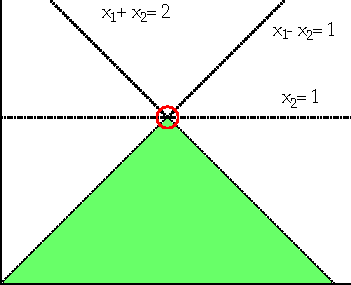
\includegraphics{./images/degenerateSystem.pdf}
\end{minipage}
\hfill
\begin{minipage}[hbt]{0.4\linewidth}
\begin{align*}
x_2 + x_3 &= 1\\
x_1 - x_2 +x_4 &=0\\
x_1 + x_2 +x_5 &= 2\\
\end{align*}
\end{minipage}
\caption{An example for a degenerate system}
\label{Fig:degenerateSystem}
\end{figure}

The system in figure \ref{Fig:degenerateSystem} gives us the solution $(1,1,0,0,0)$ for three bases $\{1,2,3\}$, $\{1,2,4\}$, $\{1,2,5\}$. This happens because we have a point where three constraints are active, although we're in 2D. It is easy to see that if we have two bases build from indices $k\in [1,\ldots,n]$ that give us the same solution one of the $x_k$ (a basic variable) has to be zero. %easy to see :S

%figure
Note that degeneracy is not a purely \emph{geometric property} (representation independend). However if a basic feasible solution of a particular standard form representation of a polyhedron $P$ is degenerated, then it is degenerated under all standard form representations of $P$.


\paragraph*{The simplex algorithm} works by moving from corner to corner, always in the direction of better costs. At first we'll have some simplifying assumptions, to avoid the messy details:

\begin{enumerate}
\item The LP is in standard form (for conversion see \ref{Sec:standardForm})
\item Every feasible basis $A$ is non-degenerate. A basis $B$ is non-degenerate if $\forall b:\ x_B=A^{-1}_Bb \gneq 0$. Note the difference to $x_B\geq 0$ for general basic solutions. So it is forbidden that more than $n$ (those in $B$ and $>n-m$ non-negativity) constraints are active (in $n$ dimensions they can't all be linearly independent of course). 
\item We are given an initial feasible basis
\item The feasible region of the LP is bounded
\end{enumerate}

In the next lectures we'll remove those assumptions one after the other.

An initial version of the algorithm works as follows:
\begin{center}
\begin{lstlisting}
SIMPLEX-TAKE-I(A,b,c)

B <- find some feasible basis
// B=$\{b_1,b_2,\ldots, b_m\} \subseteq [1,\ldots, n]$
repeat 
    for $j\in [1,n]\backslash B$ and  $b_i \in B$
        D = B $\cup$ j $\backslash$ $b_i$
        if D is a basis then
            $x_B$ = $A^{-1}_B$b
            $y_D$ = $A_D^{-1}b$ //a basic solution
            if ($y_D$ $\geq$ 0) //a bfs
                if($c_Dy_D < c_Bx_B$) //cheaper than $B$
                    B = D
until B hasn't changed                
\end{lstlisting}
\end{center}

We switch from a basis $B$ to a basis $D$ by removing a column $b_i$ from $B$ and putting in a replacement $j$ to get back to a (hopefully) full rank matrix $D$. We then check if $D$ is non-singular. If so it induces a basic solution, we just have to check if it's feasible. If yes we check if the cost of the new induced solution $y_D$ is better that the old $x_B$ and keep $D$ if it is an improvement.

It will later turn out that we don't actually have to check every combination for $j$ and $b_i$. The choice of $b_i$ is uniquely determined by the choice of $j$.

When we move from solution $x$ to solution $y$ we do so along some vector $d$ (s.t. $y=x+\Theta d$). Have a look at figure \ref{Fig:movingToSolutions}. We do some observations on the vector $d=(x_0,...,x_n)$. $d_k$ refers to the k-th component of $d$. 

\begin{figure}[hbt]
\begin{center}
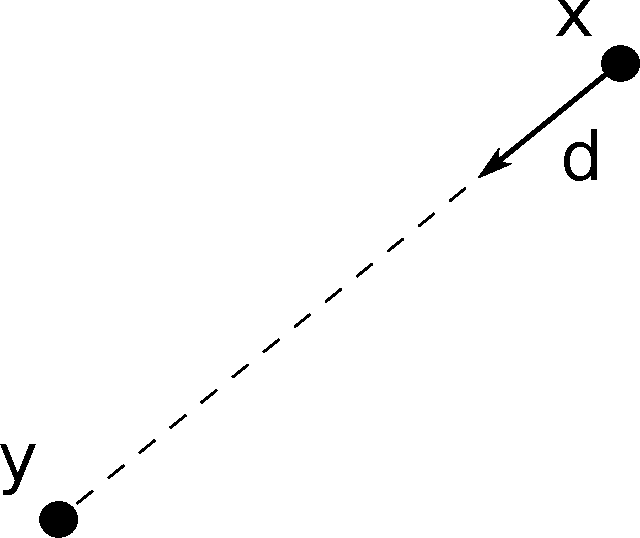
\includegraphics[width=0.3\textwidth]{./images/movingToSolutions.pdf}
\end{center}
\caption{The vector $d$ gives the direction from $x$ to $y$.}
\label{Fig:movingToSolutions}
\end{figure}

\begin{itemize}
\item $d_k=0$ if $k\not \in B \cup j$, because we assumed all non-basic variables to be zero to make the non-negativity constraints active. In particular the column $b_i$ is removed from the basis and hence the variable $x_{b_i}$ becomes $0$.

\begin{equation} d_k=0 \label{equ:dkEquZero} \end{equation}

\item $d_j>0$ let $j$ be the column added to the basis, because we made the formerly non-basic variable $x_j$ basic. That is assigning it some value $>0$. By choosing $\Theta$ accordingly we can scale this to be $d_j=1$ and make further calculations easier. Therefore we assume from now one $d_j=1$

\item Both $x$ and $y$ are bfs, i.e. both satisfy all equations. By multiplying the line equation with $A$ and solving for $Ad$: $Ad = (Ay-Ax)/\Theta = (b-b)/\Theta = 0$ we get
\begin{equation} Ad = 0 \label{equ:AdEquZero}\end{equation}
\end{itemize}

\subsubsection*{Calculating $b_i$ directly}
By using these observations we can directly calculate the $b_i$ we need to remove.

First we want to get the components $d_B$ that we don't know immediately from the above observations. We can decompose $Ad$ into the part we're looking for, $A_j d_j$ which is $A_j$ since $d_j:=1$ and $A_{\bar B} d_{\bar B}$ which is 0 since $d_{\bar B}:=0$.

\[0= Ad \sum_{i=1}^{n}A_i d_i  = \sum_{i=1}^{m}{A_{B(i)} d_{B(i)}} + A_j = A_B d_B + A_j\]

$B$ is a basis, so $A_B$ is invertible and we can compute $d_B$.

\begin{equation}
d_B = -A^{-1}_B A_j \label{equ:valueDb}
\end{equation}

The new extreme point $y$ should be a feasible solution so we also want $y\geq 0$. By plugging the calculation for $d_B$ into the equation for the line between $x$ and $y$ we get

\begin{align*}
y_B &= x_B + \Theta d_B\\
 &= x_B - \Theta A_B^{-1} A_j \geq 0
\end{align*}

We also need to ensure the nonnegativity constraints. For $x_j$ this isn't a problem as we only increase it. All nonbasic variables $x_{\bar B}$ stay at zero. So we only need to worry about the basic variables. \\ 
Remember that the basic variables in $x_B$ are all greater than 0. 
So that means if $d>0$ we are ok, however if $d_{B(i)} <0$ for some $i \in {1,...,m}$ then it can happen that we get a negative component if we choose $\Theta$ too large. We need 

\begin{center}
\begin{align*}
x_{b_i} +\Theta d_{b_i} & \geq 0\\ %was \stackrel{!}{\geq} why was it so?
\Theta &\leq \frac{-x_{b_i}}{d_{b_i}} \text{\ note: }d_{b_i}<0
\end{align*}
\end{center}

By choosing $\Theta$ sufficiently small we can avoid negativity. 

However we'd like to move as far as possible along the line $y=x+\Theta d$ without leaving the polyhedron. So we choose it like this

\[\Theta = \min_{{b_i\in B}\atop {d_{b_i} <0}} \left| \frac{x_{b_i}}{d_{b_i}}\right |\]

The variable $x_{b_i}$ that attains the above minimum will be equal to zero in $y$, i.e. in becomes non-basic and will have to be taken out of $B$. Because we assumed that the system is non degenerate there will be only one element actually attaining it or we would have a basic feasible solution with a basic variable that is 0 (and hence $>n$ constraints would be active at that solution). Also $\Theta \gneq 0$ or one of the basic variables would have been zero ($\Rightarrow x\neq y$).

Note that this was the step that assumed a bounded polyhedron. If $P$ would be unbounded and $d>0$ there could be some $x+\Theta d$ were we could move along as far as we want without leaving $P$. That would mean that $P$ contains a infinite line and is therefore not bounded (remember figure \ref{Fig:bounded_unbounded}).

\subsubsection*{Calculating the costs of the new solution}
Next we want to look at how the cost changes when going from $x$ to $y$. Again we do this by plugging in our observations into the line equation:

\begin{align*}
cy &= cx + \Theta cd\\
    &= cx + \Theta (c_Bd_B + c_jd_j) &&d_j=1\\
    &= cx + \Theta (c_Bd_B + c_j)\\
cy - cx &= \Theta (c_Bd_B +c_j)
\end{align*}

Note that using equation \ref{equ:valueDb} $c_Bd_B$ equals $- c_B A^{-1}_B A_j$.
If $y$ was a solution that we move to we did that because $cy$ was smaller than $cx$. So $c_j + c_Bd_B$ should be negative if we want to move to $y$. 

Now we know how to calculate the $b_i$ we need to remove when we put in a $j$ to get a new basis and we know a new (much more complicated, yay) criterion to check whether we move in the right direction. We combine that into a better version of the algorithm.

\begin{center}
\begin{lstlisting}
SIMPLEX-TAKE-II (A,b,c)

B = some feasible basis
repeat 
    for $j\in \{1,\ldots,n\}\backslash B$ // $b_i$ is determined
        $d_B$ = $A^{-1}_B A_j$
        if $c_j + c_Bd_B < 0$
            $b_i$ = index  s.t. $d_{b_i} <0$, 
                    minimizing $\left| \frac{x_{b_i}}{d_{b_i}}\right|$
            B = B $\cup$ j $\backslash$ $b_i$
until B hasn't changed
\end{lstlisting}
\end{center}

\subsubsection*{Reduced cost vector}
\begin{Def}[Reduced cost vector]
 Let $x$ be a basic solution, let $A_B$ be an associated basis matrix, and let $c_B$ be the vector of costs of the basic variables. For each $j$, we define the reduced costs $\bar c$ of the variable $x_j$ according to the formula 
$\bar c_j = c_j + c_Bd_B = c_j - c_B A^{-1}_B A_j$
\end{Def}


\begin{center}
\begin{lstlisting}
SIMPLEX-TAKE-III (A,b,c)

B = some feasible solution
repeat
    $\bar c$ = $c_j$ - $c_BA_B^{-1}A$ //reduced cost vector
    if $\exists j:{\bar c}_j<0$ 
        u = $A^{-1}_B A_j$ 
        if(no component of $u$ is positive)
            return 'polyhedron is unbounded'
        $b_i$ = index in B s.t. $u_i >0$ 
                minimizes  $x_{b_i}/u_i$
        B = B $\cup$ j $\backslash b_i$ 
until B hasn't changed 
// $\bar c \geq 0$ 
\end{lstlisting}
\end{center}


%alles hier haben wir schon oben bewiesen.
Let's focus on a single iteration and recapture why it works. If we start with a basic feasible solution $Ax=b, x\geq 0$, $B$ is a basis; then 

\begin{enumerate}
\item $Ay=b$, since 
\[Ay=A(x+\Theta d) = Ax + \Theta Ad = b+\Theta(A_j+A_Bd_B) = b+\Theta(A_j - A_BA_B^{-1}A_j) = b\]
Note that $A_BA_b^{-1}$ equals the identity matrix
\item $y\geq 0$. There are three cases

\begin{itemize}

\item $y_k, k\not \in B\cup j$
\[y_k=x_k+\Theta d_k = x_k = 0\]
Since $d_k=0$ as $k \not \in B$ (see formula \ref{equ:dkEquZero}) for the same reason $x_k=0$ (it isn't a basic variable therefore we set it to zero). 

\item $y_k, k=j$
\[ y_k = x_j + \Theta d_j = 0 + \Theta d_j \Rightarrow  \Theta d_k \geq 0\]
By definition of $\Theta$ %TODO which is in this case?

\item $y_k,k\in B$
\[y_k=x_k+\Theta d_k\]
This is only interesting if $d_k<0$. In that case we defined $\Theta$ to be $\min_{{b_i\in B}\atop {d_{b_i} <0}} \left| \frac{x_{b_i}}{d_{b_i}}\right |$. And hence we stay positive.

\end{itemize}

\item $D$ is a basis. Assume otherwise. Then the new vector must break the linear independence

\[A_j= \sum_{b_k\in B\backslash b_i} \lambda_k A_{b_k}\]

Since we have $d_B=-A_B^{-1}A_j$ we get

\[d_B = -\sum \lambda_k A_B^{-1} A_{b_k} \qquad \Rightarrow d_{b_i} = 0\] %TODO check this. My notes don't show the -

Which is a contradiction %ausführen
\end{enumerate}

For all these things we don't use the assumption that the system is nondegenerate. We'll use that later, when we remove that constraint. However we need that if we want to show that we always improve the objective value.

The return statement 'polyhedron is unbounded' was added to work around assumption 4. If we reach that return value we know that the costs are decreasing as $c_j < 0$ and that at no time a constraint is going to be violated, as $u$ has no positive components and therefore $\theta=\infty$ and the optimal cost equal $-\infty$.

If the assumptions hold, simplex always terminates, since there are only finitely many candidate solutions and we always increase the objective value.

\begin{thm}\label{Pr:simplexIIIopt} Let B be a basis. If $x_B=A^{-1}_Bb\geq 0$ and $\bar c=c- c_B A_B^{-1}A_j \geq 0$ then the basic feasible solution induced by $B$ is optimal.\end{thm}

\begin{pr}[Theorem \ref{Pr:simplexIIIopt}] Let $x$ be the basic feasible solution induced by $B$, $y$ be any other feasible solution. We want to argue that the cost of $x$ is smaller than the cost of $y$. %Let $d=y-x$ then 
Consider the direction $d=x-y$. From the feasibility of $x$ and $y$ it follows by using the formula \ref{equ:AdEquZero} that

\[0=Ad=A_b d_b + \sum_{k \not \in B } {A_k d_k} \Rightarrow d_b = - \sum_{k \not \in B}{A_{B}^{-1}A_k d_k}\]

Now the difference in cost between $y$ and $x$ is 
\[cd=c_{B} d_b + \sum_{k \not \in B} {d_k c_k}= \sum_{k \not \in B} {\underbrace{d_k}_{y_k-x_k\geq 0} \underbrace{(c_k-c_BA_{B}^{-1} A_k)}_{\bar c_k\geq 0}}=\sum_{k \in B} {d_k \bar c_k}\]

Notice that for all $k \in B$ we have $x_k=0$ and $y_k \geq 0$ and therefore $d_k \geq 0$. By our assumption, all reduced costs are non-negative. Thus, $c y - c x = c d \geq 0$. Sine this holds for all feasible $y$, it follows that $x$ is indeed optimal.
\end{pr}

\begin{cor}
Given that our initial four assumptions hold. Algorithm three returns an optimal feasible solution after a finite number of steps.
\end{cor}